\documentclass[twocolumn,10pt]{asme2ej}

\usepackage{epsfig} %% for loading postscript figures
\usepackage{amsmath} %for matrix

\title{Internet of Things (IoT) Application for Searching Victims}
%%{Unmaned Aerial Vehicle (UAV) Application for Fire Disaster Response}
%%% first author
\author{M. Rosyidi, Ratih H. Puspita, Shigeru Kashihara, and Fall Doudou\\
	NAIST Graduate School of Information Science\\
}


\begin{document}
	
	\maketitle    
	
	%%%%%%%%%%%%%%%%%%%%%%%%%%%%%%%%%%%%%%%%%%%%%%%%%%%%%%%%%%%%%%%%%%%%%%
	\begin{abstract}
		{\it  Fire disasters occur around the world and represent an important factor that affects human life and development. The problems start with the physical extent of the disaster, where the most important issue is preserving human lives. Currently, efforts are aimed at recognizing and forecasting the possibility that a disaster will happen, reacting in an efficient manner to the disaster when it happens, and quickly and efficiently assessing the damage to guide in fixing and restoring the normal state. Internet of Things (IoT) system application can assist monitoring and management of fire disaster. They can gather information and data captured in the current area. The system control center can analyze transmitted data and present useful information to determine the current situation in a disaster area. There are two main works of this research. The first is Aerial Photography which identifying the damage situation in an affected area, and the second is Wi-Fi Sensing which locating vulnerable people in the affected area.
			
			\textbf{Key words:} Fire disarter, Internet of Things, Aerial Photography, Wi-Fi Sensing
		}
	\end{abstract}
	
	\section{Introduction}
	
	Fires are the most frequently occurring accidents, with diverse causes, frequent destruction of buildings, and high threats to human safety. For example, forest fires usually occur in hot, dry areas that do not get much rain. They can break out when the trees and the ground get really dry and hot. Sometimes lightning strikes the trees and starts a fire that could spread for miles.  They spread quickly lighting trees, brushes, grass, and houses. They can most easily spread in the forest area. Facing wildfires can be very dangerous and is not recommended.
	
	The Fire and Rescue Services responded to a multiplicity of events such as major disasters, large building fires, Hazmat incidents and environmental events such as flooding and forest fires, and in doing so, they have a range of tools and equipment that they can call on to assist in the firefighting effort. With a fast response time and increasing sensing capability, Internet of Things (IoT) can be very useful for area detection of the fire disaster. In this way, IoT is an emerging technology that is revolutionizing a variety of applications, from commerce and recreation to military and safety \cite{Faisal}. 
	
	The vast deployment of IoT-enabled devices (often battery powered and able to operate and transmit wirelessly) could bring benefits in terms of data network resilience in face of disaster. For rescue operations, the fire department needs to gather information about such vulnerable people, in addition to information about the damage situation in the affected area. By used IoT to gather this information is more efficient and safer than gathering the information manually. IoT devices could enable limited communication services which can be used for fire detection, intervention monitoring, and also for post-fire monitoring \cite{Restas} \cite{Zeinab}.
	
	Today, the technology for position tracking has been widely used. The technology uses the Global Positioning System (GPS) owned by the Government of the United States. The GPS can be used to find the current position, address or direction to a place. Devices that have both GPS and Wi-Fi sensor can be used to send information about a network back to a GPS company so that they can determine where the network is. The way this works is by having the device send the access point's BSSID (MAC address) along with the location determined by GPS. When GPS is used to determine the location of a device, it also scans nearby networks for publicly accessible information that can be used to identify the network. Once the location and nearby networks are found, the information is recorded real time. The next time someone is near one of those networks but they don't have great GPS signal, the service can be used to determine an approximate location since the network's location is known\cite{Sheng}. 
	
	Data obtained from the sensor in real time then put into a database server over the network using Raspberry Pi. The data can be accessed in real time via a web server. Raspberry Pi is a base station consisting of database servers and web servers built on computer hardware platforms. This makes Raspberry Pi has a complexity that is not high so it is easy to develop, and does not consume high costs.
	
	The focus of this research is how to increase human safety because even if we have conducted evacuation drills when a disaster strikes, it can be difficult to guarantee human safety because fires are such unpredictable events. This is especially true for vulnerable persons, such as old persons, differently able persons, small children, and babies, who are prone to receive damage. This research will combine the current technology of IoT with a system application that can gather information about victims of a fire accident. Internet of Things (IoT) system application can assist monitoring and management of fire disaster. They can gather information and data captured in the current area. The system control center can analyze transmitted data and present useful information to determine the current situation in a disaster area. There are two main works of this research. The first is Aerial Photography which identifying the damage situation in an affected area, and the second is Wi-Fi Sensing which locating vulnerable people in the affected area.
	
	%%%%%%%%%%%%%%%%%%%%%%%%%%%%%%%%%%%%%%%%%%%%%%%%%%%%%%%%%%%%%%%%%%%%%%
	\section{Related Work}
	\subsection{Internet of Things (IoT)}
	Internet of Things (IoT) is a concept that aims to expand the benefits of continuously connected internet connectivity. As for capabilities such as data sharing, remote control, and so on, including also on objects in the real world. Examples of food, electronics, collectibles, any equipment, including living things that are all connected to local and global networks through embedded and always on censorship. Essentially, the Internet of Things refers to objects that can be uniquely identified as virtual representations in an Internet-based structure. Many predict that the Internet of Things (IoT) is "the next big thing" in the world of information technology. This is because a lot of potential that can be developed with the technology of the Internet of Things (IoT) is \cite{Zeinab}.
	
	An IoT device has a radio that can send and receive wireless connections. The IoT wireless protocol is designed to meet several basic services, operate with low power and bandwidth, and work in mesh networks. Some devices work at 2.4 GHz field frequencies, which are also used by Wi-Fi and Bluetooth, and sub-GHz coverage. The sub-GHz frequencies including 868 and 915 MHz have an advantage in low interference. The method used by the Internet of Things is wireless or automatic control without distance. Implementation of the Internet of Things itself usually always follow the developer's desire in developing an application that he created, if the application was created to help to monitor a room then the implementation of the Internet of Things itself must follow the flow of programming diagrams about the sensor in a house, how far the distance room can be controlled, and internet network speed used. The development of network and Internet technologies such as the presence of IPv6, 4G, and Wimax, can help the implementation of the Internet of Things become more optimal, and allow the distance can be passed further, making it easier for us to control things\cite{Zeinab}.
	
	%%%%%%%%%%%%%%%%%%%%%%%%%%%%%%%%%%%%%%%%%%%%%%%%%%%%%%%%%%%%%%%%%%%%%%
	\subsection{Raspberry Pi}
	Raspberry Pi used as a single board computer for docking and processing wifi sensor, camera, and GPS.It's low-cost computer capable of running a GNU/Linux desktop environment on a low-power ARM processor. All port on Raspberry Pi capable for running three sensors that will be used in this research. RPi port can handle camera and wifi sensor and GPS will communicate using GPS Hat that compatible with Rasberry PI. Data sensor will be collected simultaneously and battery powerful enough to handle raspberry PI movement of drone flying arround the location of the disaster area. The position of the GPS module paired to Raspberry Pi which is a microcomputer that also has a digital port input/output such as on the microcontroller board with a GPS module support tool used as GPS signal capture to obtain a coordinate that will be displayed on the MAP in the form of tracking results. Development of the GPS system is based on NMEA data format processed to become coordinate data and stored in the Raspberry Pi database.The processed NMEA formats are GPGGA and GPRMC. In format GPGGA contains position data i.e. latitude, longitude, altitude, and UTC Time, whereas in format GPRMC contains RTC update data (Real Time Clock)\cite{Yuyang}.
	
	\subsection{Related Research}
	Song Gao and Sathya Prasad \cite{Song} discussed about employing spatial analysis in indoor positioning and tracking using Wi-Fi access points. In the paper, they proposed a novel Wi-Fi indoor positioning and tracking framework. A mobile indoor positioning application developed as a proof of concept. The proposed methodology and theoretical framework can guide engineers to implement cost-effective indoor positioning infrastructure. Sheng-Cheng Yeh et.al. \cite{Sheng} discused about a study on outdoor positioning technology using GPS and Wi-Fi networks. This paper mention that the pattern matching method that takes the Received Signal Strength Indicator (RSSI) at the receiving end as the fingerprinting is one of the key technologies. In addition, they proposed a positioning technology based on a portable mobile device with GPS and Wi-Fi based Pattern Matching Method to design a Selective Weighting Method in order to improve the precision of positioning under NLOS outdoor environment. S.R.Vijayalakshmi \cite{Vijayalakshmi} was discussed about the requirements of user and key main issues of wireless sensor network hardware and software for fire monitoring system. In addition, they were discussed application features of IoT technology and Wireless Sensor Network technology for according to fire monitoring system. This paper proposed a new fire monitoring fire system software platform and development proposition.  
	
	%%%%%%%%%%%%%%%%%%%%%%%%%%%%%%%%%%%%%%%%%%%%%%%%%%%%%%%%%%%%%%%%%%%%%%
	\section{System Model}
	\subsection{Design of IoT Application}
	The IoT application system for searching victims are required a Raspberry Pi B+, wireless sensor, GPS, antenna, battery, and mobile device to support our system model. Wireless sensor which connected to raspberry pi collect the signal strength against distance. Fig. 1 describes the general work flow of our system.
	
	\begin{figure}[t]
		\begin{center}
			\setlength{\unitlength}{0.012500in}%
			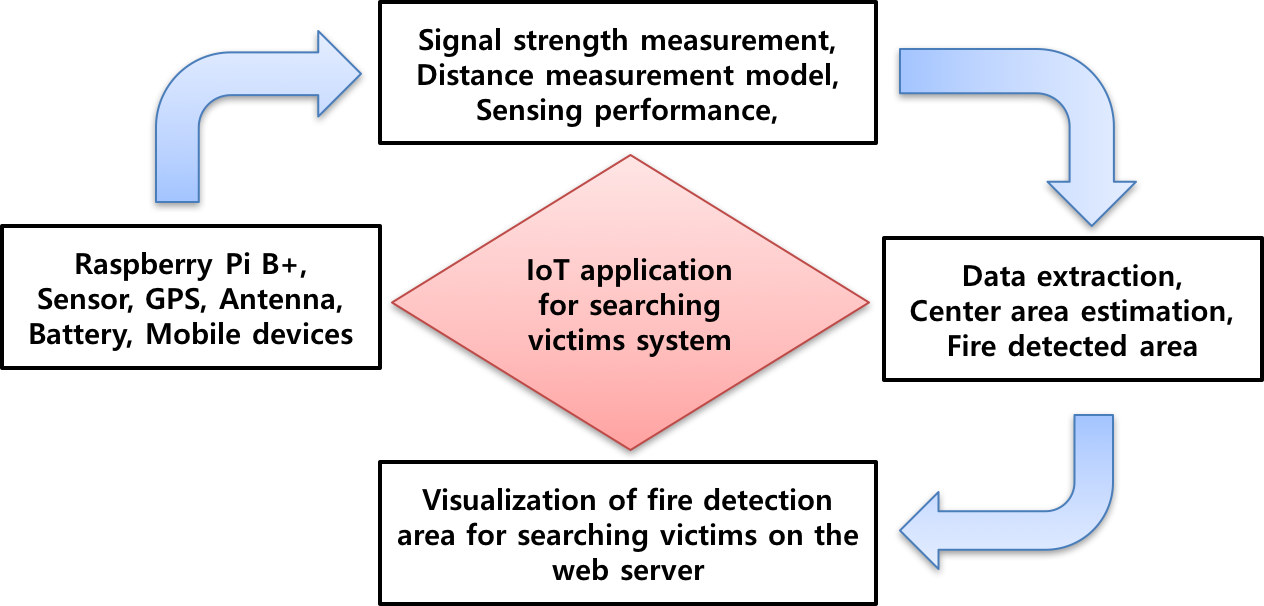
\includegraphics[width=0.5\textwidth,height=50mm]{WorkFlow.png}
		\end{center}
		\caption{Work Flow of IoT Application for Searching Victims}
		\label{Work_Flow} 
	\end{figure}
	
	In the fire disaster area, the UAV application can identify and locate Wi-Fi packets sent from vulnerable people's smartphones. Afterward, we identify potential locations of vulnerable people, as the invisible information of the fire disaster area. Fig. 2 shows the general system model of this works, where we connected the Raspberry Pi B+ with GPS and Wi-Fi device. Afterward, to connect the Raspberry Pi B+ to the camera, we were added push button in order to we run automatically based on the button pressed.
	
	\begin{figure}[t]
		\begin{center}
			\setlength{\unitlength}{0.012500in}%
			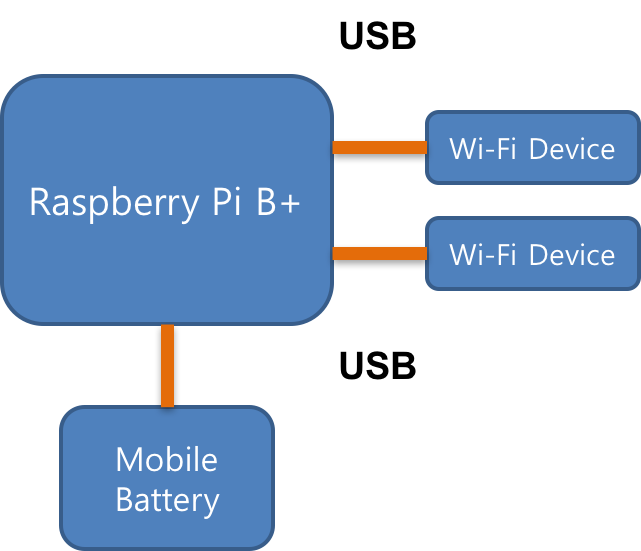
\includegraphics[width=0.3\textwidth,height=50mm]{Fig1_SystemModel}
		\end{center}
		\caption{System Model of Wifi Sensing}
		\label{System_Model} 
	\end{figure}
	
	\subsection{Data Collection}
	\subsubsection{Signal Strength Measurement}
	\textbf{Fundamentals for Wifi measuring:} the distance between the transmitter and the receiver has an important role in determining the position. In contrast to GPS, WiFi, at a time measurement method, does not come into question, since such an exact time is difficult to achieve synchronization. In addition, the path from space to the ground is much farther than from one access point to a mobile user. The received signal strength indicator (RSSI) and the signal noise ratio (SNR) are the most suitable \cite{Yuyang}. 
	
	\textbf{Signal Strength:} the signal strength is measured in dBm (decibel in milliwatt). A Wifi station has a EIRP (Equivalent isotropically radiated power) of 100mW - 1000mW (20dBm - 30dBm) \cite{Yuyang}.
	\begin{equation}
	Lp(dBm) = 10 * log \frac{P}{1mW}
	\end{equation}
	The signal strength measurements scenario can be seen in Fig. 3, where we collected the RSSI from iPhone mobile user in distance 0-70m. 
	\begin{figure}[t]
		\begin{center}
			\setlength{\unitlength}{0.012500in}%
			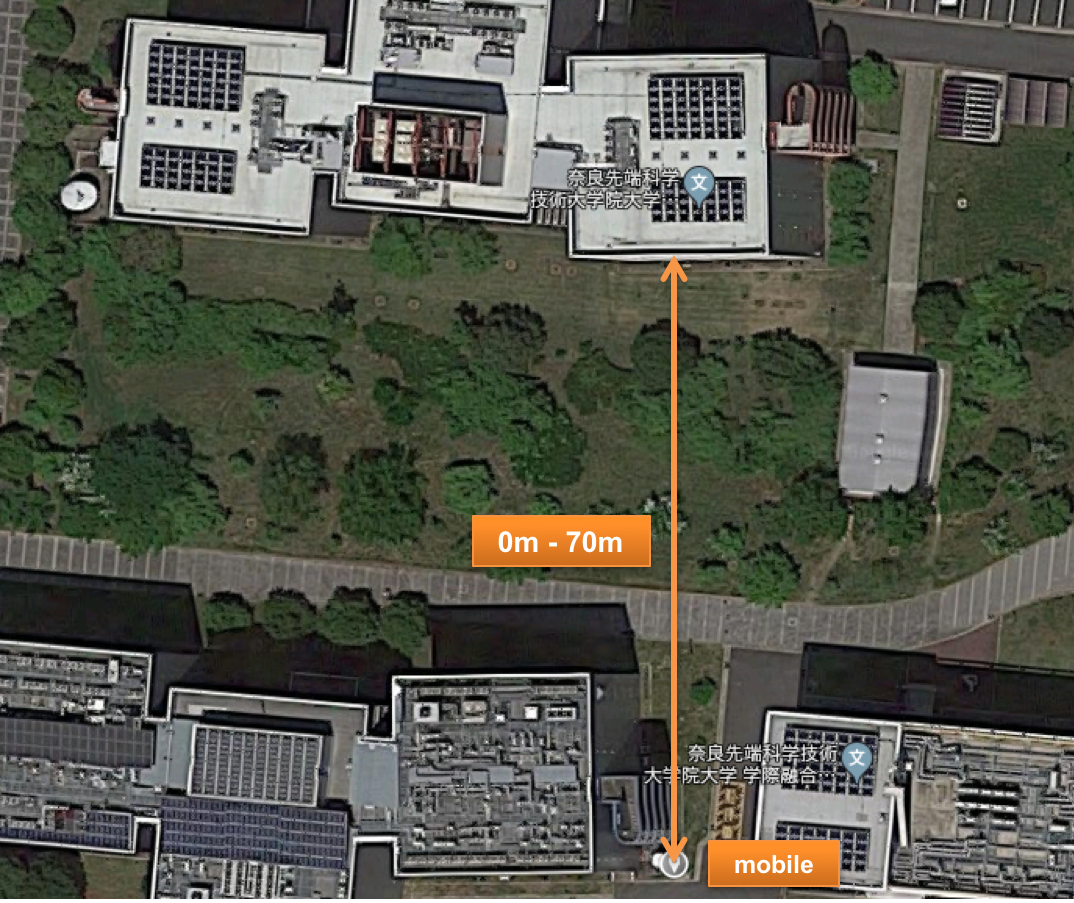
\includegraphics[width=0.4\textwidth,height=35mm]{Fig3_2SigScenario}
		\end{center}
		\caption{Signal Strength Measurements Scenario}
		\label{RSSI Scenario} 
	\end{figure}
	
	\subsubsection{Distance Measurement Model}
	After we were collected the RSSI, we had decided the distance between wifi sensor and mobile devide for each RSSI value. According to our measurements, we had RSSI on a certain range for each distance. Afterward, we need to average the RSSI by applied linier regression equation, which stated as 
	\begin{equation}
	Y = a + bX
	\end{equation}
	where $Y$ is the predicted dependent variable, $X$ is an independent variable that has a certain value, $a$ is the $y$-intercept and $b$ is the slope of the line. Fig. 4 plots the linear regression of RSSI against distance.
	\begin{figure}[t]
		\begin{center}
			\setlength{\unitlength}{0.012500in}%
			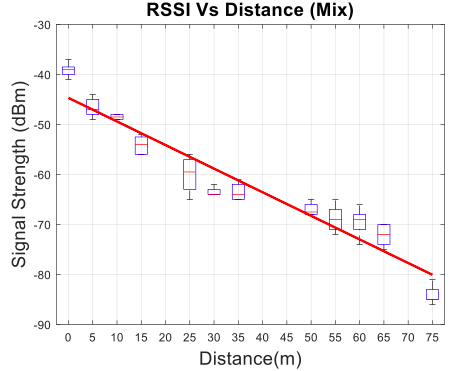
\includegraphics[width=0.4\textwidth,height=50mm]{Fig4_RegLin.png}
		\end{center}
		\caption{Linear Regression of RSSI against Distance}
		\label{Linear} 
	\end{figure}
	The boxplot represents the range of RSSI value, and the red line represents linear regression of RSSI value. And this regression value used to obtain an average value of RSSI for each distance. By used linear regression, we obtained the distance measurement model of our mobile device. We used iPhone and Android for the measurement, and we obtain the distance measurement model as
	\begin{eqnarray}
	y_{iPhone} = -0.45x - 45.15 \\
	y_{Android} = -1.33x - 14.67
	\end{eqnarray}
	where $y$ is distance estimation, and $x$ is signal strength measurement.
	
	\subsubsection{Spherical Theory for Positioning}
	In this research, we assume that earth follows the spherical theory.Information latitude and longitude from GPS sensor must be converted to the Earth reference system to axis values (x,y,z) in the cartesian coordinate system as follow \cite{Song}:
	
	\begin{eqnarray}
	x &= R * cos(lat) * cos(lon) \notag \\
	y &= R * cos(lat) * sin(lon) \notag \\
	z &= R * sin(lat) 
	\end{eqnarray}
	
	R is the approximate radius of the earth (e.g., 6371km), we try to find the center of coordinate as position of the personal mobile user that involved in fire accident. Three position of wifi is enough to measure the center and estimate the radius of the selected area. 
	
	============== Under Revision ==================
	
	\subsection{Area Estimation}
    \subsubsection{Center Area Estimation}
    Three position of wifi-sensor from device will be converted to the cartesian of earth $(x,y,z)$. Distance of each coordinate to the center of earth represented as radius of earth, this corresponds to the spherical theory of earth. Position of Wi-Fi sensors defined by :

    \begin{gather}
    2
    \begin{bmatrix}
    \begin{array}{llll}
    x_1 & y_1 & z_1\\
    x_2 & y_2 & z_2\\
    x_3 & y_3 & z_3\\
    \end{array}
    \end{bmatrix}
    \begin{bmatrix}
    \begin{array}{llll}
    x\\
    y\\
    z\\
    \end{array}
    \end{bmatrix}
    =
    \begin{bmatrix}
    \begin{array}{llll}
    2R^2-d1^2\\
    2R^2-d2^2\\
    2R^2-d3^2\\
    \end{array}
    \end{bmatrix}
    \end{gather}

    ${(x1,y1,z1),(x2,y2,z2),(x3,y3,z3)}$ represents the cartesian of three position of wifi sensor against a mobile device, while $(x,y,z)$ is cartesian variable of mobile device possibility position. To obtain the actual position that represent latitude and longitude we must follow

	\begin{eqnarray}
	p = (180/\pi)*arcsin(z/R) \\
	q = (180/\pi)*arctan(y/x)
	\end{eqnarray}
    where $p$ is latitude of center area estimation and $q$ is longitude of center area estimation.

	\section{Evaluation}
	\subsection{Methodologies}
	\subsubsection{Limitation}
	GPS and Wi-Fi sensor running alongside, we can get the measure of system route and be sensing the position of the mobile user that detected during the experiment. We were considering an iPhone mobile device measurement. For this experiment, we put an iPhone on the ground floor to capture the signal strength / RSSI and determine the distance. We were circling the area 4 times to capture the RSSI of the iPhone. A plenty of RSSI data captured and collected in the experiment. After the RSSI collected and separated in accordance with device type, RSSI data is averaged for each device to determine the nearest point to the actual device location. The nearest point here represents as center data estimation for the distance of the mobile device. From that center estimation, we were grouping the data by position. According to the specification of the GPS accurately, in the certain distance GPS will detect the same Coordinate (latitude and longitude). In this experiment condition, sometime there are several RSSI detected in same area Coordinat. Fig. 4 describes the RSSI grouped in the same Coordinates. There are 5 group captured from the experiment.   
	
	\subsubsection{Positioning Algorithm}
	The center data estimation obtained by referring to 3 point/node with 3 strongest RSSI value.  
	Afterward, we selected three positions/node of the measurement from an iPhone to estimate the center of the estimated area by used the mathematical model (7) and (8).
	
	\begin{figure}[t]
		\begin{center}
			\setlength{\unitlength}{0.012500in}%
			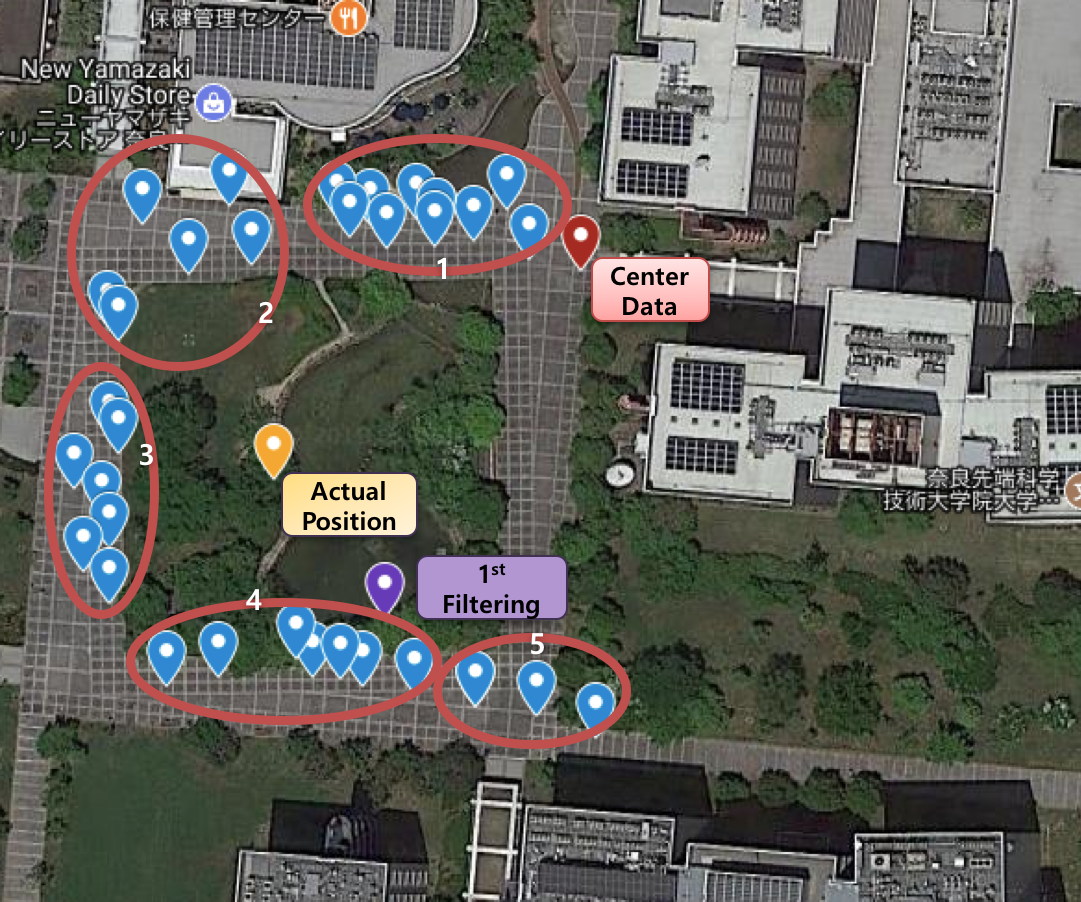
\includegraphics[width=0.4\textwidth,height=40mm]{GroupingData.png}
		\end{center}
		\caption{Grouping All RSSI Data to Determine the Location of Center Estimation}
		\label{Experiment Route} 
	\end{figure}
	
	
	\begin{figure}[t]
		\begin{center}
			\setlength{\unitlength}{0.012500in}%
			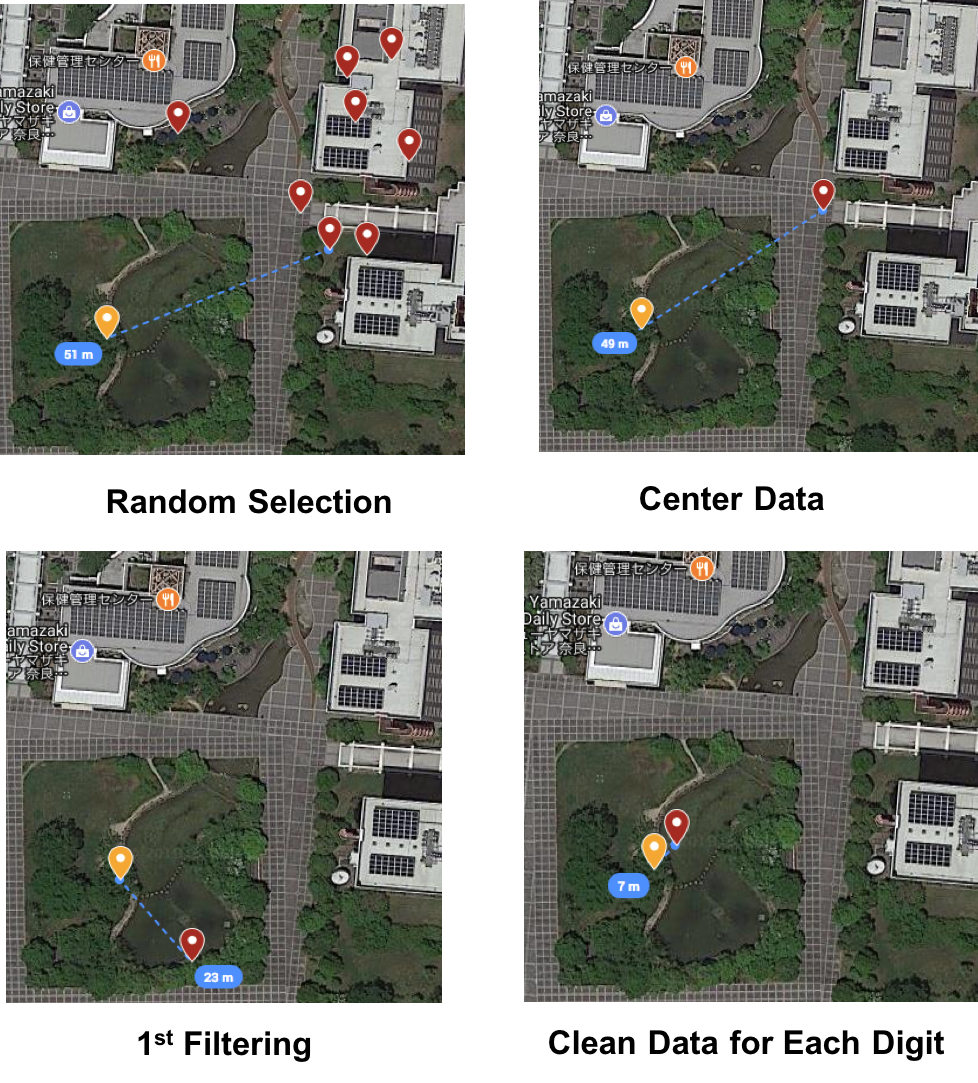
\includegraphics[width=0.5\textwidth,height=60mm]{ComparisonMethod.png}
		\end{center}
		\caption{Comparison the Position of Center Estimation}
		\label{Experiment Route} 
	\end{figure}
	
	\subsubsection{Single Device}
	After we obtained the center of area estimation, we visualized area into the Google Maps API. Area estimated divided into three categories. According to Fig.6, blue area indicates the assumption of strong signal position area of the mobile user with radius 10m, green area indicates the medium signal position area with radius 20m, and red area indicates the weak signal position area with radius 30m. Assumption area color related to the priority for searching people that involved in the fire accident. From the result of our experiment, the location of iPhone detected in the green area with radius 20m.
	\begin{figure}[t]
		\begin{center}
			\setlength{\unitlength}{0.012500in}%
			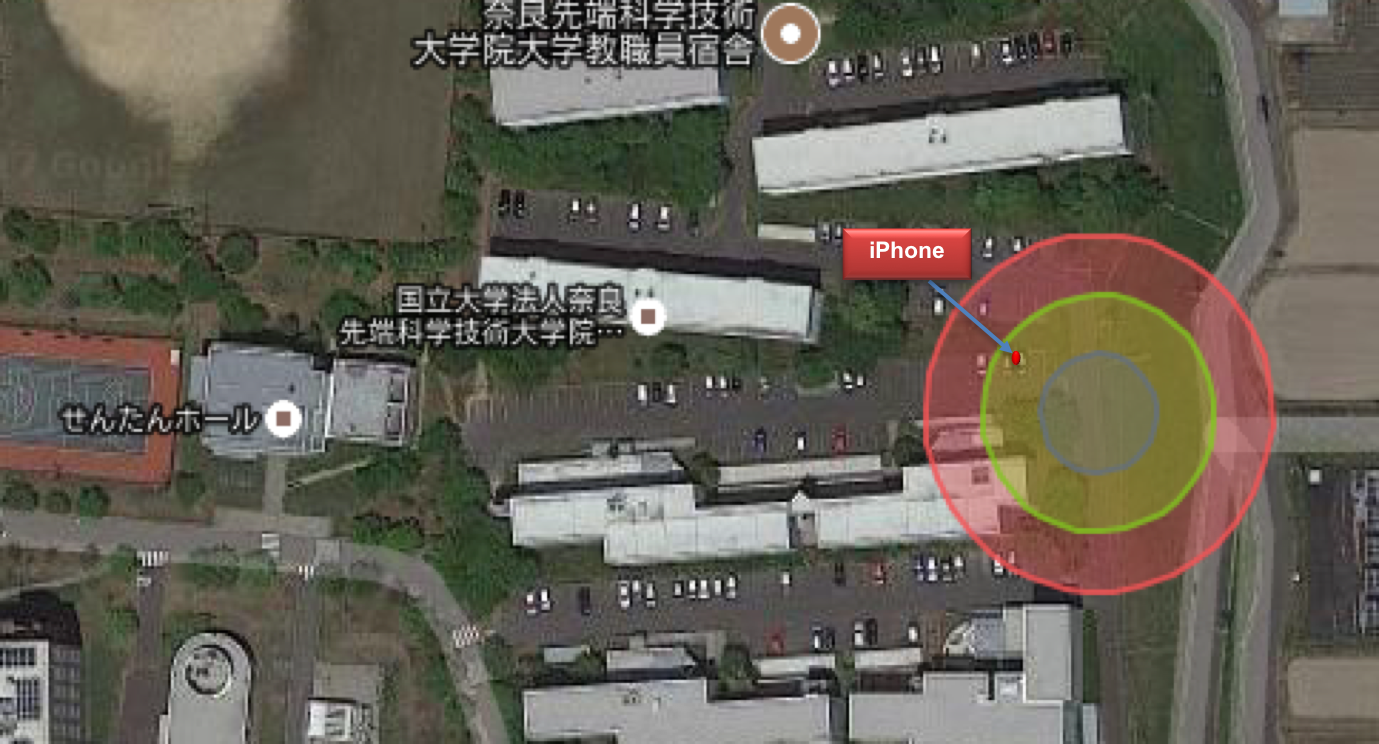
\includegraphics[width=0.4\textwidth,height=40mm]{Fig5a_AreaDetected.png}
		\end{center}
		\caption{Estimated Area of Single Device}
		\label{Area Detection} 
	\end{figure}
	
	\subsubsection{Multi-Device}
	Beside by used single device, we were also conduct the experiment in multi-device. For this experiment, we put several mobile phones (iPhone and Android) scattered around the experiment route which describes with a yellow line in the Fig. 7. We were collected the RSSI data for all mobile device. 
	
	In the next step, we obtained the distance between grouped RSSI each data and center estimation. In this step, we set the distance limitation condition based on the requirement of wifi sensing maximum distance which detected. And in this experiment, we set the required distance in 100m. In the other words, we used all the data which has obtained distance less than 100m. After that, we selected the minimum distance as the center area estimation for each device by used mathematical model (7) and (8). As the final step, we visualized area into the Google Maps which showed in Fig. 7. Fig. 7 describes that we detected 9 kinds of mobile device. Similarly, from the previous section, Area estimated divided into three categories. They are blue area indicates the assumption of strong signal position area of the mobile user with radius 10m, green area indicates the medium signal position area with radius 20m, and red area indicates the weak signal position area with radius 30m.
	
	\begin{figure}[t]
		\begin{center}
			\setlength{\unitlength}{0.012500in}%
			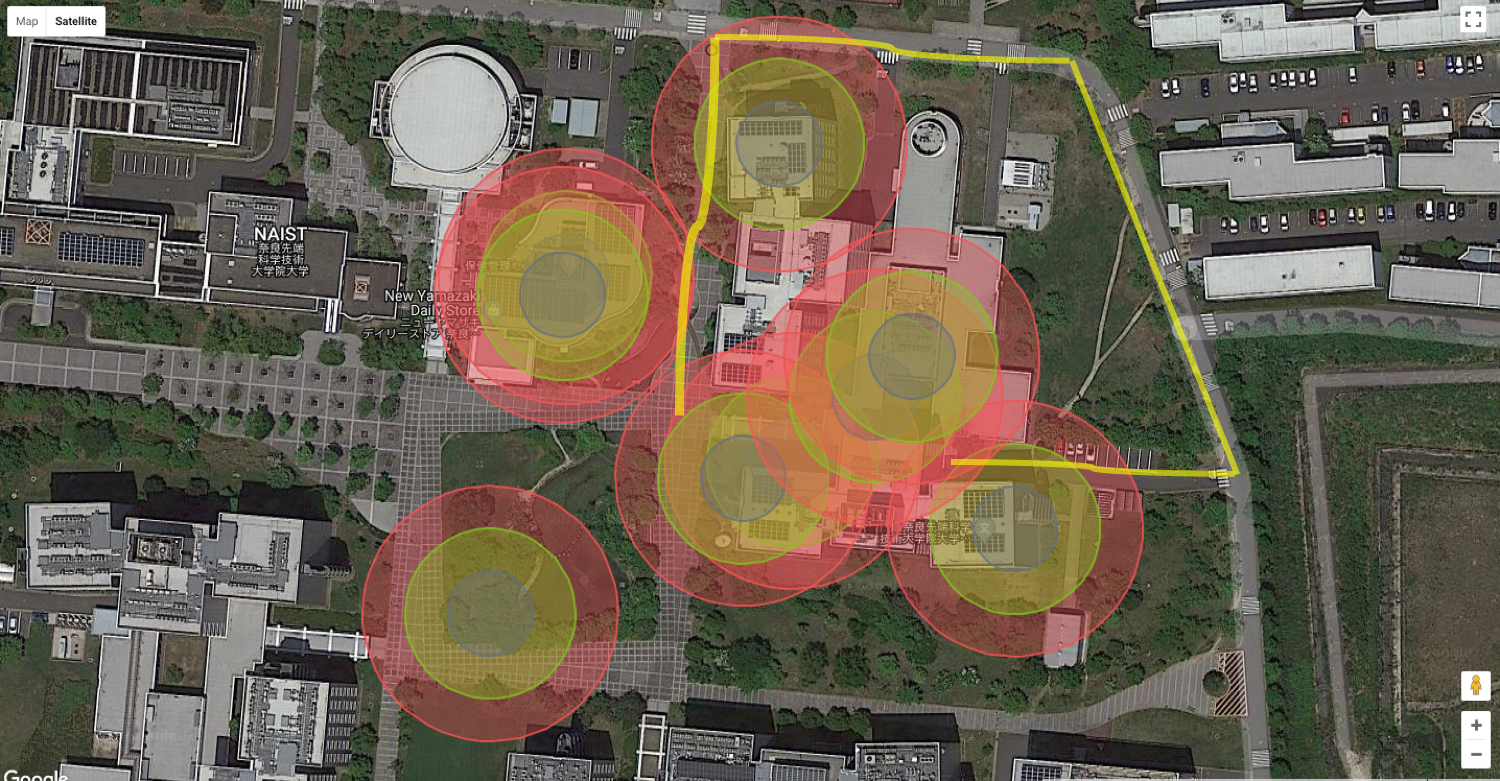
\includegraphics[width=0.4\textwidth,height=40mm]{Fig7_AreaDetected_MultiDevice.png}
		\end{center}
		\caption{Estimated Area of Multi Device}
		\label{Experiment Route} 
	\end{figure}
	
	\section{Conclusions and Future Works}
	This paper studied GPS and WiFi calculates better positioning accuracy to estimate the fire disaster area. Based on the experiment, we collected the signal strength to determine the distance against RSSI. Afterwards, we obtained the center area detected and determined the radius between mobile device and wi-fi sensor. We were devide the area into 3, they are strong signal (r=10m) with blue color, medium signal (r=20m) with green color, and weak signal (r=30) with red color. Our experiment show that the mobile device (iPhone) located in the green area with r=20m.
	
	In future work, we need to consider the different type of device used. Perform the measurement for any device and create general calculation of distance base on signal strength that obtains from the experiment.The other hand, break the limitation of error signal strength is a very important thing to get the center area estimation accurately. 

	\begin{acknowledgment}
		
	First and foremost, we would like to thank God Almighty (Allah SWT) for giving us the strength, knowledge, and opportunity to undertake this research. We send our gratitude to the supervisor, Assistant Professor Shigeru Kashihara and Assistant Professor Fall Doudou, for his guidance and providing us with an excellent atmosphere for doing research. We would like to offer my special thank to all members of this project who also supporting to finish this project.
		
	\end{acknowledgment}
	
	%%%%%%%%%%%%%%%%%%%%%%%%%%%%%%%%%%%%%%%%%%%%%%%%%%%%
	\begin{thebibliography}{99}
		\bibitem{Faisal}
		Faisal Arain and Shahab Moeini. Leveraging on Unmanned Ariel Vehicle (UAV) for Effective Emergency Response and Disaster Management. 2005
		
		\bibitem{Restas}
		Restas, Agoston. Drone Applications for Supporting Disaster Management, \textit{World Journal of Engineering and Technology}, 2015.
	
		\bibitem{Zeinab}
		Zeinab Kamal Aldein Mohammeda and Elmustafa Sayed Ali Ahmedb, Internet of Things Applications, Challenges and Related Future Technologies, \textit{World Scientific News 67(2) 126-148}, February, 2017.
		
		\bibitem{Sheng}
		Sheng-Cheng Yeh, Wu-Hsiao Hsu, Ming-Yang Su, Ching-Hui Chen, and Ko-Hung Liu, A Study on Outdoor Positioning Technology Using GPS and WiFi Networks, \textit{IEEE International Conference on Networking, Sensing and Control}, Okayama, Japan, March 26-29, 2009.
				
		\bibitem{Yuyang}
		Yuyang Huang, Li-Ta Hsu, Yanle Gu, Haitao Wang, and Sunsuke Kamijo, How Wi-Fi Location Services Work, \textit{IEICE Trans Fundamentals}, Vol. E99-A, No. 9, September, 2016.
		
		\bibitem{Song} 
		Song Gao, Sathya Prasad. Employing Spatial Analysis in Indoor Positioning and Tracking Using Wi-Fi Access Points, 2016.
		
		\bibitem{Vijayalakshmi} 
		S.R.Vijayalakshmi and S.Murugunand. Internet of Things Technology for Fire Monitoring System, \textit{International Reserach Journal of Engineering and Technology (IRJET)}, June, 2017.
		
		\bibitem{Masellis}
		Masellis M., Ferrara M.M., Gunn S.W.A. FIRE DISASTER AND BURN DISASTER: PLANNING AND MANAGEMENT, Annals of Burns and Fire Disasters - vol. XII - no. 2, June, 1999.
		
		\bibitem{Seung}
		Seung-Hyun Seo, Jung-In Choi and Jinseok Song, Secure Utilization of Beacons and UAVs in Emergency Response Systems for Building Fire Hazard, September, 2017.
		
		
	\end{thebibliography}
	
\end{document}
